%part 2

	\chapter{Прохождение критической энергии в регулярной магнитооптической структуре синхротрона}\label{ch:transition}

\par Данная глава посвящена рассмотрению а) влияния критической энергии на продольную динамику, а также б) процедуры скачка критической энергии в регулярной структуре синхротрона. Учтены высшие порядки, а также рассмотрены модели импеданса для различных интенсивностей сгустка.

\par Исходя из изложенных уравнений продольного движения в Главе \ref{ch:dual}, приближение энергии пучка к критическому значению ведет к изохронному движению, при котором частота синхротронных колебаний стремится к нулю и означает отсутствие продольного перемешивания частиц в сепаратрисе. При этом нарушается адиабатичность движения, а также становится значительным влияние высших порядков разброса по импульсу, что приводит к нелинейности движения. При этом затухание Ландау оказывается неспособно подавить возникающие возмущения в интенсивных сгустках. Наличие пространственного заряда и других импедансов оказывает влияние на развитие продольной микроволновой неустойчивости, нестабильности отрицательной массы и поперечной неустойчивости голова-хвост (head-tail) \cite{ng}, \cite{MetralMohl} и в конечном счёте приводит к потере фазовой стабильности.

\par	Традиционно критическая энергия преодолевается с помощью процедуры её скачка \cite{risselada:jump}. При этом изменяются параметры ускорителя для внесения соответствующего возмущения и резкого кратковременного скачка критической энергии в момент близости энергии сгустка к критическому значению. После скачка, параметры установки возвращаются к исходному значению до скачка с поправкой на увеличившуюся энергию пучка. Однако, сложностью является непосредственное создание скачка с заданной величиной и темпом, что не всегда легко реализуемо. Возможный способ создания скачка критической энергии состоит в изменении количества бетатронных колебаний или набега фазы, поскольку в случае регулярной структуры критическая энергия пропорциональна горизонтальной частоте колебаний $\gamma_{\text{tr}} \sim \nu_{x}$. Такой метод может быть реализован путем создания возмущения в квадруполях. Этот подход был применен в 1969 году на установке PS (Proton Synchrotron), CERN \cite{cern:q-jump}. Однако, его применение существенно ограничено возможностью сдвига рабочей частоты и тем самым устанавливает предел на величину скачка, а скорость изменения -- на темп скачка. Другой метод основан на кратковременном возмущении дисперсионной функции, путем установки специальных квадруполей обратных полярностей, расположенных через один период друг от друга.  Таким образом, происходит искажение дисперсии без сдвига частоты бетатронных колебаний. Такой метод реализован позднее в 1974~году, также в PS \cite{cern:new-jump} и позволяет достигнуть большей величины и темпа измерения критической энергии.

\par Прохождение критической энергии является актуальной задачей для протонного пучка в строящемся комплексе NICA-Nuclotron (ОИЯИ г. Дубна). С целью изучения данной проблемы, исследована динамика продольного движения в окрестности критической энергии У-70 (НИЦ “Курчатовский институт”~--~ИФВЭ г. Протвино). Численно промоделирована процедура скачка критической энергии в синхротроне У-70. Полученные данные также апробированы на ускорительном сеансе \cite{Kolokolchikov:2025_U70}.

\par Важным фактором, описывающим взаимодействие пучка и элементов ускорителя является влияние различного рода импедансов, а также типов высокочастотных резонаторов (ВЧ) на продольную динамику во время процедуры преодоления критической энергии. Отличительной особенностью является использование ВЧ барьерного типа, в результате чего достигается равномерное распределение пучка в фазовом пространстве. \cite{hans:bb}.

\par Результаты данного исследования помогут осветить потенциальные последствия прохождения критической энергии и определить существенные параметры, влияющие на динамику фазового движения.

	\section{Построение регулярной структуры на основе ячеек ФОДО, ФДО, ОДФДО}\label{sec:transition_jump/FODO_FDO}



\begin{figure} [h!]

   \includegraphics*[width=.32\columnwidth]{2_twiss_fodo_cell.pdf}
   \includegraphics*[width=.32\columnwidth]{2_twiss_fdo_cell.pdf}
   \includegraphics*[width=.32\columnwidth]{2_twiss_odfdo_cell.pdf}

   \includegraphics*[width=.32\columnwidth]{2_twiss_fodo_regular.pdf}
   \includegraphics*[width=.32\columnwidth]{2_twiss_fdo_regular.pdf}
   \includegraphics*[width=.32\columnwidth]{2_twiss_odfdo_regular.pdf}

   \caption{Твисс-параметры $\beta_{x,y}$, $D_{x}$. Сверху -- для ячеек для синглетной ФОДО, дублетной ФДО, триплетной ОДФДО ячеек; посредине -- регулярная структура; снизу -- резонансная.}
   \label{fig:fodo_fdo_odfdo_regular}
\end{figure}

\par На основе ФОДО, ФДО и ОДФДО ячеек могут быть сконструированы регулярные поворотные арки как показано на рис. \ref{fig:fodo_fdo_odfdo_regular}. Для ФОДО-ячейки характерно наибольшее пространственное разделение минимумов и максимумов бета-функций. При этом именно в ФОДО-структуре достигаются максимальные значения как бета-функции, так и дисперсионной функции. Следует отметить, что величина градиента в квадрупольных линзах, необходимая для обеспечения одинакового набега фазы, возрастает в следующем порядке: ФОДО, ФДО, ОДФДО. 

	\subsection{Подавление дисперсии в регулярных арках с missing magnet и/или квадруполями с варьируемыми градиентами}\label{sec:transition_jump/suppression}

\par Дисперсионная функция $D(s)$ является решением неоднородного уравнения поперечного движения и характеризует смещение замкнутой орбиты для частиц с ненулевым относительным разбросом по импульсу $\delta$ \cite{lee}.

\par Необходимость наличия бездисперсионных областей возникает во многих задачах ускорительной техники. Так, в коллайдерных экспериментах пучки сталкиваются в заданной точке (Interaction Point, IP), где для достижения требуемой светимости необходимо обеспечить минимальный поперечный размер пучка, прямо пропорциональный значению дисперсионной функции. При инжекции из бустера (booster) в основное кольцо (main ring) требуется согласование Твисс-функций для сохранения пучка; выполнение этого условия существенно упрощается в случае нулевой дисперсии, тогда как при её наличии приходится искусственно возбуждать орбиту для согласования. Кроме того, размещение определённых элементов, например высокочастотных резонаторов, в бездисперсионных точках позволяет минимизировать эффект синхро-бетатронной связи.

\par Наиболее простым способом дисперсия в поворотной арке может быть подавлена в периодичной структуре, где частота кратна целому числу $2\pi$. При таком подходе создаётся ахромат первого порядка. Другим известным, уже ставшим классическим, является подход с введением техники отсутствующих магнитов ('missing magnet') \cite{autin:dispersion}. В этом случае, не реализуются условия ахромата первого порядка. Так в коллайдере NICA реализована техника отсутствующих магнитов и инжекция происходит в место с ненулевой дисперсией, что обусловлено особенностью расположения оборудования.

\par Особо стоит отметить, что в случае спиновой динамики, на прямом участке необходимо использование прямых фильтров Вина, что будет показано в Главе \ref{ch:EDM}. Такое устройство не возмущает орбиту так как изначально планируется сделать нулевую силу Лоренца (или одинаковую кривизну полей E и B полей). Однако, при этом искажается дисперсионная функция, что должно быть дополнительно компенсировано.

	
	\section{Прохождение критической энергии}\label{sec:transition_jump/U-70}
	
	\subsection{Численное моделирование динамики продольного движения} \label{sec:transition_jump/modeling}
	
\par Основные уравнения, которые будут проанализированы – уравнения продольного фазового движения.
Классически уравнения \ref{eq:long_motion_eq_n} могут быть записаны в зависимости от времени:
	
\begin{equation}
\begin{cases}
\begin{aligned}
& \dv{\tau}{t}=\eta(\delta) \cdot \frac{h \cdot \Delta E}{\beta^2 \cdot E_0}, \\
& \dv{(\Delta E)}{t}=\frac{V(\tau)}{T_0}.
\end{aligned}
\end{cases}
\label{eq:long_motion_eq_t}
\end{equation}	

\noindent Для моделирования приведенной системы уравнений используются различные программы. В работе используется  BLonD \cite{blond}. Для пересчёта временной задержки могут быть использованы 2 различные схемы: как 'простая', учитывающая только первый порядок разложения $\eta$:

\begin{equation}
\Delta t^{n+1}=\Delta t^n+\frac{\eta_0^{n+1} T_0^{n+1}}{\left(\beta_s^{n+1}\right)^2 E_s^{n+1}} \Delta E^{n+1},
\label{eq:blond_dt_simple}
\end{equation}

\noindent так и 'точная', учитывающая зависимость от высших порядков разложения: 

\begin{equation} \label{eq:blond_dt_exact}
\begin{aligned}
 \Delta & t^{n+1}=\Delta t^n+T_0^{n+1}\times\\
& \times \left[\left(1+\alpha_0^{n+1} \delta^{n+1}+\alpha_1^{n+1}\left(\delta^{n+1}\right)^2+
\alpha_2^{n+1}\left(\delta^{n+1}\right)^3\right)\left(\frac{1+\frac{\Delta E^{n+1}}{E_s^{n+1}}}{1+\delta^{n+1}}\right)-1\right].
\end{aligned}
\end{equation}

\noindent Для пересчёта приращения энергии используется уравнение, включающее учёт только гармонических ВЧ, а также разности энергии $n$ и $n+1$ оборота:

\begin{equation} \label{eq:blond_dE}
\Delta E^{n+1}=\Delta E^n+\sum_{k=0}^{n_{\mathrm{rf}-1}-1} V_k^n \sin \varphi_{\mathrm{rf}, k}\left(\Delta t^n\right)-\left(E_s^{n+1}-E_s^n\right).
\end{equation}

\noindent Такой подход затрудняет моделирование барьерного ВЧ в BLonD; при этом барьер представляется в виде набора ВЧ-станций с различными частотами, соответствующими Фурье-разложению сигнала. Этот метод будет использован в дальнейшем.
	
	\subsection{Стабильность продольного фазового движения вблизи критической энергии}\label{sec:transition_jump/adiabaticity}
	
\par Уравнения \ref{eq:long_motion_eq_t} определяют продольные колебания с определенной частотой. Вдали от критической энергии частота синхротронных колебаний слабо меняется со временем, движение адиабатично. Вблизи критической энергии нарушается условие адиабатичности синхротронного движения. Характерное время адиабатичности можно оценить, сравнивая синхротронную частоту с темпом изменения удерживающей сепаратрисы, что показано на рис. \ref{fig:adiabatic_time_nonlin_time}a \cite{ng}:

\begin{equation}
\tau_{\textrm{ad}}=\left(\frac{\pi\beta^2mc^2\gamma_{\textrm{tr}}^4}{\dot{\gamma}\omega_0^2heV\left|\cos{\phi_{\textrm{s}}}\right|}\right)^{1/3},
\label{eq:adiabaticity}
\end{equation}

\noindent где $\gamma_{\textrm{tr}}$ – Лоренц-фактор, соответствующий критической энергии, $\dot{\gamma}$ – темп изменения энергии. При адиабатичном движении как сепаратриса, так и частота колебаний медленно меняется со временем.

\par Нелинейность продольного движения проявляется когда $\eta_1\delta$ сравнимо с $\eta_0$; характерное время (рис. \ref{fig:adiabatic_time_nonlin_time}б):

\begin{equation}
\tau_{\textrm{nl}}=\frac{\eta_1\hat{\delta}}{\sfrac{2\dot{\gamma}}{{\gamma_{\textrm{tr}}}^3}}=\gamma_{\textrm{tr}}\frac{\sfrac{3}{2}\beta^2+\gamma_{\textrm{tr}}^2\alpha_1}{2\dot{\gamma}}\
\label{eq:nonliniarity}
\end{equation}

\noindent где $\hat{\delta}\approx{10}^{-2}-{10}^{-3}$ -- абсолютное значение максимального отклонения импульса вблизи критической энергии, $\alpha_1$ -- второй порядок коэффициента уплотнения орбиты. Для регулярной ФОДО структуры У-70 с скомпенсированной натуральной хроматичностью, получено $\alpha_1\simeq0.01$ \cite{Kolokolchikov:2025_U70}.

\begin{figure}
   \includegraphics*[width=0.49\columnwidth]{3_adiabatic_time.png}
   \includegraphics*[width=0.49\columnwidth]{3_nonlin_time.png}
   \caption{а) Классическая синхротронная частота и темп изменения огибающей сепаратрисы в окрестности критической энергии от номера оборота; б) изменение первого и второго порядков коэффициента проскальзывания $\eta_0$, $\eta_1\delta$ в окрестности критической энергии от номера оборота.}
   \label{fig:adiabatic_time_nonlin_time}
\end{figure}

\par Кроме того, из ур. \ref{eq:long_motion_eq_t} следует условие стабильности синхротронных колебаний

\begin{equation}
\eta_0\cos\phi_{\text{s}}<0.
\label{eq:long_stability}
\end{equation}

\noindent Видно, что для продольного согласования при прохождении критической энергии должна быть сдвинута фаза $\phi_{\textrm{s}}$ ускоряющего поля ВЧ, на величину $\pi-2\phi_{\textrm{s}}$.

\par Оценки для У-70, приведенные в таблице \ref{tab:u-70}, отражают тот факт, что время адиабатичности (ур. \ref{eq:adiabaticity}) может быть сравнимо со временем нелинейности (ур. \ref{eq:nonliniarity}) $\tau_{\textrm{ad}}\sim\tau_{\textrm{nl}}$. При приближении энергии к критическому значению, продольная длина пучка уменьшается, а разброс по импульсам увеличивается. На рис. \ref{fig:3_eta} приведены результаты моделирования прохождения критической энергии при ускорении от $7.0$ до $13.0$ ГэВ для $\eta=\eta_0$ и $\eta=\eta_0+\eta_1\delta$ в различных моделях BLonD. Влияние второго порядка коэффициента проскальзывания увеличивает продольный эмиттанс, что может быть критично и приводит к необходимости применения дополнительных мер по сохранению фазового объёма.

\begin{table}
\begin{center}
\begin{tabular}{| m{10cm} | M{2.5cm} |}
\hline Полная длина $L$, м  & 1483.699 \\
Коэффициент расширения орбиты $\alpha_0$ & 0.011120 \\
Коэффициент расширения орбиты $\alpha_1$ & 0.01 \\
Критическая энергия, ГэВ & 7.957 \\
Лоренц-фактор $\gamma_{\mathrm{tr}}$ & 7.48 \\
Максимальная интенсивность в сеансе, ppp & $4 \cdot 10^{12}$ \\
Ускоряющая фаза $\sin \left(\phi_{\mathrm{s}}\right.$) & $1 / 2$ \\
Время адиабатичности $\tau_{\mathrm{ad}}$, мс & 3.218 \\
Время нелинейности $\tau_{\mathrm{nl}}$, мс & 2.646 \\
Гармоническое число & 30 \\
Амплитуда ускоряющих станций, кВ & 10 \\
Количество ускоряющих станций & 40 \\
Темп ускорения $\dot{\gamma}, \mathrm{c}^{-1}$ & 42.7 \\
\hline
\end{tabular}
\end{center}
\caption{Основные параметры кольца и ВЧ для синхротрона У-70}
\label{tab:u-70}
\end{table}

\begin{figure}
   \includegraphics*[width=0.32\columnwidth]{3_eta_beam_lenght.png}
   \includegraphics*[width=0.32\columnwidth]{3_eta_energy_spread.png}
   \includegraphics*[width=0.32\columnwidth]{3_eta_emit.png}
   \caption{Зависимость a) длины сгустка, б) разброса энергии внутри сгустка, в) продольного эмиттанса от номера оборота в окрестности критической энергии при изменении энергии от $7$ до $13$ ГэВ для трёх моделей без скачка и учёта импеданса. 
Синяя – учёт только первого порядка $\eta=\eta_0$, ‘simple’ solver, оранжевая – $\eta=\eta_0$, ‘exact’ solver, зеленая – $\eta=\eta_0+\eta_1\delta$, ‘exact’ solver.}
   \label{fig:3_eta}
\end{figure}

\subsection{Влияние индуктивного импеданса}

\par На продольную динамику также оказывают влияние элементы ускорителя. Для описания электромагнитного взаимодействия пучка с элементами структуры ускорителя вводится понятие импеданса \cite{laclare:inst}. Он зачастую представляется достаточно сложной функцией, содержащей как мнимую, так и действительную часть. Вид импеданса может быть определен как аналитически, взяв во внимание все наиболее значимые элементы, так и экспериментально, на уже действующей установке. Поскольку оба эти подхода являются достаточно комплексными и сложными, в качестве первого приближения могут быть использованы простые модели импедансов.
\par Особенно важным для изучения продольной динамики при прохождении критической энергии является продольный импеданс $Z_\parallel\left(\omega\right)$. В данной работе ограничимся исследованием динамики с учётом его мнимой индуктивной компоненты $\sfrac{Z_n}{n}=\pm i \cdot const$. Положительная индуктивность может соответствовать продольному импедансу связи пикап-электродов, кикер-магнитов и сильфонов \cite{pashkov:transition}. Отрицательная индуктивность соответствует импедансу гладкой камеры при наличии пространственного заряда и описывается аналитически:

\begin{equation}
\frac{Z_{\textrm{SC}}}{n}=-\frac{Z_0}{2\beta\gamma^2}\left[1+2\ln{\left(\frac{b}{a}\right)}\right].
\label{sc}
\end{equation}

\noindent Для наглядности, приведём напряжение, индуцированное про\-стран\-стве\-нным зарядом, $V_{\mathrm{SC}}(\phi)$. Уравнение определяется производной от функции распределения $f(\phi)$ в пространстве \cite{weilee:sc}:

\begin{equation}
V_{\text{SC}}\left(\phi\right)=\frac{Z^2h^2g_0Z_0ce}{2R_0\gamma^2}\cdot\frac{\partial\left(N_0\cdot f\left(\phi\right)\right)}{\partial\phi}.
\label{eq:V_sc}
\end{equation}

\par На сеансе для У-70 наблюдалась интенсивность в импульсе порядка $N_{\textrm{tot}}=4\cdot{10}^{12}$ ppp (particles per period). Соответственно в сгустке – порядка $N_{\textrm{beam}}=4\cdot{10}^{11}$ ppb (particles per beam). Моделирование продольной динамики при изменении энергии от 7 до 9 ГэВ показывает, что при малой интенсивности $N_{\textrm{beam}}=4\cdot{10}^{11}$ ppb как для отрицательного, так и для положительного значений рассматриваемого импеданса пучок сохраняет стабильность. Для больших интенсивностей $N_{\textrm{beam}}=1\cdot{10}^{12}$ ppb наблюдается существенное изменение симметрии фазового объёма и увеличение продольного эмиттанса (рис. \ref{fig:3_wo_jump}, табл. \ref{tbl:u-70_crossing}). В соответствии с экспериментальными данными начальное значение длины сгустка $\tau_L=4t_\sigma\simeq20$ нс для $E_0=7$ ГэВ. Для гауссова распределения $\Delta E_{0} = 4E \sigma = 52.7$ МэВ, $\varepsilon_{0}^{95\%}=1.23$ эВ$\cdot$с.
	
\begin{figure} [h!]
   \includegraphics*[width=0.32\columnwidth]{3_wo_jump_beam_lenght.png}
   \includegraphics*[width=0.32\columnwidth]{3_wo_jump_energy_spread.png}
   \includegraphics*[width=0.32\columnwidth]{3_wo_jump_emit.png}
   \caption{Зависимость a) длины cгустка, б) разброса энергии внутри сгустка, в) продольного эмиттанса от номера оборота в окресности критической энергии при изменении энергии от $7$ до $9$ ГэВ без скачка, с учётом различного вида импеданса и интенсивностей.}
   \label{fig:3_wo_jump}
\end{figure}

\begin{table}
\begin{center}
\begin{tabular}{| m{4cm} | M{2.5cm} | M{2.5cm} | m{6.6cm} |}
\hline 
Параметры моделирования & $95 \%$ фазовый объем, $\text{эВ}\cdot\text{с}$ & Сохранение пучка & Особенности \\
\hline
$\alpha_1=0, \text { simple, }$ Без импеданса & 1.23 & $100\%$ & Простая модель, рост эмиттанса отсутствует \\
\hline 
$\alpha_1=0, \text { exact, }$ Без импеданса & 1.4 & $99.65\%$ & Точная модель, нелинейность отсутствует, влияние неадиабатичности, рост эмиттанса \\
\hline 
$\alpha_1=0.01, \text { exact, }$ Без импеданса & 1.8 & $99.65\%$ & Влияние нелинейности, рост эмиттанса в $\sim 1.5$ раза \\
\hline 
$
 \alpha_1=0.01, \text { exact, }$
$ Z_n / n=-i \cdot 10, \quad$
$4 \cdot 10^{11} \mathrm{ppb} $
 & 1.8 & $99.65\%$ & Уменьшение длины сгустка после $\gamma_{\mathrm{tr}}$, фокусирование после $\gamma_{\mathrm{tr}}$, рост эмиттанса \\
\hline 
$
\alpha_1=0.01, \text { exact, }$ 
$ Z_n / n=+i \cdot 10, \quad$
$4 \cdot 10^{11} \mathrm{ppb} $
 & 1.9 & $99.60\%$ & Уменьшение длины сгустка до $\gamma_{\mathrm{tr}}$, раскачивание после $\gamma_{\mathrm{tr}}$, рост эмиттанса \\
\hline 
$
\alpha_1=0.01, \text { exact, } $ 
$Z_n / n=-i \cdot 10, \quad$
$1 \cdot 10^{12} \mathrm{ppb}$
 & 2.3 & $99.60\%$ & Существенное сжатие длины сгустка до $\gamma_{\mathrm{tr}}$, рост эмиттанса \\
\hline 
$
 \alpha_1=0.01, \text { exact, } $ 
$ Z_n / n=+i \cdot 10, \quad$
$ 1 \cdot 10^{12} \mathrm{ppb}$
 & 4.1 & $98.60\%$ & Увеличенная амплитуда квадрупольных колебаний, существенный рост эмиттанса \\
\hline
\end{tabular}
\end{center}
\caption{Результаты численного моделирования прохождения критической энергии, в том числе с учётом влияния различных импедансов для различных интенсивностей.}
\label{tbl:u-70_crossing}
\end{table}


\newpage
\subsection{Процедура скачка критической энергии}

\par Для сохранения стабильности продольного движения, продольный эмиттанс не должен расти при прохождении критической энергии. Для этого используется метод скачка критической энергии при приближении энергии пучка к критическому значению \cite{risselada:jump}. Такой подход заключается в быстром изменении параметров ускорителя, при котором изменяется коэффициент уплотнения орбиты $\alpha$, связанный с $\gamma_{\textrm{tr}}$ (ур.~\ref{eq:alpha}). В общем случае коэффициент расширения орбиты определяется как интеграл:

\begin{equation}
\alpha=\frac{1}{C} \int_0^{\mathrm{C}} \frac{D(s)}{\rho(s)} d s,
\label{eq:alpha_general}
\end{equation}

\noindent где $s$ -- переменная длины ускорителя, $D\left(s\right)$ -- дисперсионная функция, $\rho\left(s\right)$ -- кривизна орбиты. Изменение коэффициента расширения орбиты в стационарной установке возможно при модулировании дисперсионной функции, так как $\rho\left(s\right)$ остается неизменной. 

\par Таким образом, увеличивается скорость прохождения критической энергии, при этом темп ускорения остаётся неизменным. Параметры скачка определяются исходя из особенностей магнитооптической структуры и возможности изменения тока во вспомогательных квадрупольных линзах либо в квадруполях, расположенных в поворотных арках. Оба подхода будут рассмотрены далее на примере скачка критической энергии в синхротронах У-70 и NICA.

\section{Особенности процедуры скачка критической энергии в синхротроне У-70}

\par Модуляция дисперсионной функции в синхротроне У-70 осуществляется вспомогательными квадруполями во $2$-ом и $8$-ом блоках каждого суперпериода \cite{cherniy:ihep}. На рис. \ref{fig:3_twiss_U70} изображены параметры Твисса для одного суперпериода, состоящего из 10 магнитных блоков с совмещённой функцией как для полностью регулярной структуры У-70, так и структуры с искаженной дисперсионной функцией.

\begin{figure} [h!]
   \includegraphics*[width=0.49\columnwidth]{3_twiss_U70_regular.png}
   \includegraphics*[width=0.49\columnwidth]{3_twiss_U70_modulated.png}
   \caption{Твисс-параметры $\beta_x,\beta_y, D_x$ для суперпериода У-70 a) регулярная структура; б) структура с модулированной дисперсией.}
   \label{fig:3_twiss_U70}
\end{figure}

\par Вспомогательные квадруполи расположены через полпериода $\Delta\nu_{x,y}=0.5\times0.5$ и имеют противоположные полярности. При такой модуляции дисперсии не происходит сдвига рабочей точки, поскольку действие одного квадруполя, подавляется другим в силу указанного набега фазы. В таблице \ref{tab:jump} приведены значения рабочей точки в ходе процедуры поднятия критической энергии и скачка.   
Рассматриваемый скачок имеет асимметричный характер, поднятие критической энергии на переднем фронте происходит на $\Delta \gamma_{\textrm{tr}}=0.9$ за $36$ мс, а сам скачок — за $1$ мс на заднем фронте. Принципиальная схема процедуры и соответствующее изменение первого порядка коэффициента скольжения приведены на рис. \ref{fig:3_gamma_transition_jump_U70}. Процедура скачка на сеансе У-70 приведена на рис. \ref{fig:3_jump_U70_oscilogram}а, продольная линейная плотность сгустка относительно фазы ВЧ в момент скачка отражена на рис. \ref{fig:3_jump_U70_oscilogram}б

\begin{table}
\begin{center}
\begin{tabular}{| M{5cm} |c|c|}
\hline 
Время от момента инжекции, мс & Рабочая точка $\nu_{x, y}$ & Относительно скачка \\
\hline
290 & $9.921 \times 9.842$ & До процедуры \\
295 & $9.917 \times 9.808$ & Начало процедуры \\
310 & $9.849 \times 9.787$ & Середина процедуры \\
326 & $9.780 \times 9.771$ & Момент скачка \\
330 & $9.902 \times 9.809$ & После \\
\hline
\end{tabular}
\end{center}
\caption{Изменение рабочей точки в процессе процедуры скачка критической энергии на У-70.}
\label{tab:jump}
\end{table}

\begin{figure}
   \includegraphics*[width=0.49\columnwidth]{3_gamma_transition_jump_U70.png}
   \includegraphics*[width=0.49\columnwidth]{3_eta0_jump_U70.png}
   \caption{a) Поднятие критической энергии при процедуре скачка; б) соответствующее изменение первого порядка коэффициента скольжения $\eta_0$.}
   \label{fig:3_gamma_transition_jump_U70}
\end{figure}

\begin{figure}
   \includegraphics*[width=0.49\columnwidth]{3_jump_U70_oscilogram.png}
   \includegraphics*[width=0.49\columnwidth]{3_jump_U70_beam_profile.png}
   \caption{а) Скачок критической энергии на сеансе У-70. Зеленая линия – сигнал с фазового датчика, фиолетовая – градиент в обмотках дополнительных квадруполей, голубая – сигнал с пикового детектора; б) Продольная линейная плотность сгустка относительно фазы ВЧ в момент скачка.}
   \label{fig:3_jump_U70_oscilogram}
\end{figure}

\par Результаты моделирования продольного движения (рис. \ref{fig:3_jump} и табл. \ref{tab:u-70_model}) показаны для разных моделей при ускорении от $6.9-12.9$ ГэВ для скачка критической энергии. А также для скачка с учётом импедансов вида $\frac{Z_n}{n}=\pm i\cdot const$ и разных интенсивностей при ускорении $6.9-8.9$ ГэВ (рис. \ref{fig:3_jump_imp}). Начальные значения $\tau_L=4t_\sigma\simeq20$ нс при $E_0=6.9$ ГэВ, $\Delta E_{0} = 4E_{\sigma} =49.3$ МэВ, $\varepsilon_{0}^{95\%}=1.16$~эВ$\cdot$с. Данные моделирования продольного движения соответствуют изменению длины сгустка в ходе ускорительного цикла на сеансе У-70 для низкоинтенсивного пучка (рис. \ref{fig:3_jump_U70_beam_lenght}).

\begin{figure}
   \includegraphics*[width=0.32\columnwidth]{3_jump_beam_lenght.png}
   \includegraphics*[width=0.32\columnwidth]{3_jump_energy_spread.png}
   \includegraphics*[width=0.32\columnwidth]{3_jump_emit.png}
   \caption{Зависимость a) длины сгустка, б) разброса энергии внутри сгустка, в) продольного эмиттанса от номера оборота в окрестности критической энергии при изменении энергии от $6.9$ до $12.9$ ГэВ для трёх моделей со скачком, без учёта импеданса. Синяя – учёт только первого порядка $\eta=\eta_0$, ‘simple’ solver, оранжевая – $\eta=\eta_0$, ‘exact’ solver, зеленая – $\eta=\eta_0+\eta_1\delta$, ‘exact’ solver.}
   \label{fig:3_jump}
\end{figure}

\begin{figure}
   \includegraphics*[width=0.32\columnwidth]{3_jump_imp_beam_lenght.png}
   \includegraphics*[width=0.32\columnwidth]{3_jump_imp_energy_spread.png}
   \includegraphics*[width=0.32\columnwidth]{3_jump_imp_emit.png}
   \caption{Зависимость a) длины cгустка, б) разброса энергии внутри сгустка, в) продольного эмиттанса от номера оборота в окрестности критической энергии при изменении энергии от $6.9$ до $8.9$ ГэВ со скачком, с учётом различного вида импеданса и интенсивностей.}
   \label{fig:3_jump_imp}
\end{figure}

\begin{figure}
   \centering
   \includegraphics*[width=0.49\columnwidth]{3_jump_U70_beam_lenght.png}
   \caption{Изменение длины сгустка в ходе ускорительного цикла на сеансе У-70.}
   \label{fig:3_jump_U70_beam_lenght}
\end{figure}

\par Сравнение двух способов прохождения критической энергии — со скачком и без него — показывает, что в случае скачка сокращение продольной длины сгустка оказывается меньше. Соответственно, воздействие рассмотренных импедансов на сгусток уменьшается. Рост эмиттанса наблюдается лишь для интенсивного сгустка с числом частиц порядка $N_{\textrm{beam}}=1\times10^{12}$ ppb.

\begin{table}
\begin{center}
\begin{tabular}{| m{4cm} | M{2.5cm} | M{2.5cm} | m{6.6cm} |}
\hline 
Параметры моделирования & $95 \%$ фазовый объем, $\text{эВ}\cdot\text{с}$ & Сохранение пучка & Особенности \\
\hline
$ \alpha_1=0, \text { simple, } $ Без импеданса
 & $1.165$ & $100\%$ &
Простая модель, рост эмиттанса отсутствует \\
\hline
$ \alpha_1=0, \text { exact, } $ Без импеданса
 & $1.167$ & $100\%$ & 
Точная модель, рост эмиттанса отсутствует  \\
\hline
$ \alpha_1=0.01, \text { exact, }$ Без импеданса
 & $1.174$ & $100\%$ & Нелинейность отсутствует, рост эмиттанса отсутствует \\
\hline 
$ \alpha_1=0.01, \text { exact, } $
$ Z_n / n=-i \cdot 10, \quad $
$ 4 \cdot 10^{11} \mathrm{ppb} $
 & $1.17$ & $100\%$ & Уменьшение длины после скачка $\gamma_{\text {tr }}$ \\
\hline 
$ \alpha_1=0.01, \text { exact, } $
$ Z_n / n=+i \cdot 10, \quad $
$ 4 \cdot 10^{11} \mathrm{ppb} $
 & $1.17$ & $100\%$ & Слабые квадрупольные колебания до скачка $\gamma_{t r}$ \\
\hline
$ \alpha_1=0.01, \text { exact, } $
$ Z_n / n=-i \cdot 10, \quad$
$ 1 \cdot 10^{12} \mathrm{ppb} $
 & $1.23$ & $99\%$ & Длина сгустка существенно сокращается, небольшой рост эмиттанса \\
\hline
$ \alpha_1=0.01, \text { exact, } $
$ Z_n / n=+i \cdot 10, \quad$
$ 1 \cdot 10^{12} \mathrm{ppb} $
 & $1.23$ & $99\%$ & Большая амплитуда квадрупольных колебаний, небольшой рост эмиттанса \\
\hline
\end{tabular}
\end{center}
\caption{Результаты численного моделирования прохождения критической энергии скачком с учетом влияния различных импедансов для различных интенсивностей.}
\label{tab:u-70_model}
\end{table}

\par Подводя итог, было рассмотрено прохождение критической энергии в гармоническом ВЧ как с использованием метода скачка, так и без него. Проведено численное моделирование продольной динамики для различных импедансов и интенсивностей сгустков; результаты апробированы на протонном синхротроне У-70. Установлено, что ключевым фактором является темп ускорения, увеличение которого достигается методом скачка. Изменение значения критической энергии реализуется посредством модуляции дисперсионной функции, что позволяет контролировать продольный эмиттанс в момент её прохождения. Изученные особенности продольной динамики представляют интерес для дальнейших исследований на комплексе NICA.

\section{Особенности процедуры скачка критической энергии в синхротроне NICA для протонного пучка}

\par Проблема прохождения критической энергии в синхротроне NICA (ОИЯИ г. Дубна) актуальна для экспериментов с протонами при энергии пучка $12.4$ ГэВ, поскольку может приводить к росту эмиттанса и в конечном счёте накладывает ограничения на конечную светимость. Для экспериментов с тяжелыми ионами при энергии $4.5$ ГэВ такой сложности не возникает, так как критическая энергия, характеристика кольца, составляет $5.7$ ГэВ. 

\par В регулярной структуре NICA реализация скачкообразного прохождения критической энергии со сдвигом бетатронной частоты ограничивает величину возможного скачка. Это связано с тем, что скорость изменения градиентов квадруполей задаёт предельный темп изменения критической энергии. Подобная схема была проанализирована как для барьерной, так и для гармонической ВЧ-станций, различающихся по принципу действия. Также выполнено сравнение с методикой скачка критической энергии, реализованной на синхротроне У-70.

\par Магнитооптическая структура поворотных арок NICA состоит из $12$ ФОДО ячеек с подавленной на краях дисперсией методом отсутствующих магнитов. С помощью программ численного моделирования движения пучка в магнитных системах ускорителей MADX \cite{madx} и OptiM \cite{optim} изучена зависимость изменения критической энергии от частоты бетатронных колебаний, при этом изменялся градиент в фокусирующих квадрупольных линзах. Именно в этих элементах расположен максимум $\beta_x$ и $D_x$. Как видно из рис. \ref{fig:tr_nica}, в имеющейся структуре $\Delta\gamma_{\textrm{tr}}=1.1\Delta q$. Максимальная вариация частоты или рабочей точки составляет $\pm\Delta q=0.05$, что соответствует измерению критической энергии порядка $\Delta\gamma_{\textrm{tr}}=0.09$. Соответствующее суммарное изменение градиента $\Delta Kl=4\pi\Delta q\beta_{\textrm{a}}~=~0.055$~м$^{-1}$, где $\beta_{\textrm{a}}=11.5$ м – средняя бета-функция. Тогда максимальное изменение градиента в одном квадруполе $\Delta G = \Delta Kl(BR/N_{\textrm{F}}l)=0.5$ Тл/м, где $N_{\textrm{F}}=24$ – количество фокусирующих линз, $B\rho=22$ Тл$\cdot$м – магнитная жесткость при энергии протонов $5.7$ ГэВ (критическая энергия), $l=0.47$ м – длина квадруполя. При этом ограничение скорости нарастания тока приводит к ограничению в изменении градиента квадрупольных линз. Темп изменения критической энергии $\dv*{\gamma_{\textrm{tr}}}{t}=8.5$ c$^{-1}$ \cite{Syresin:2021_polar}.

\begin{figure}[!h]
   \includegraphics*[width=.49 \columnwidth]{3_gamma_tr_vs_dQF}
   \includegraphics*[width=.49 \columnwidth]{3_tunes_vs_dQF}
   \caption{Зависимость критической энергии и рабочей точки от возмущения градиента квадрупольных линз.}
   \label{fig:tr_nica}
\end{figure}

\begin{figure}[!h]
   \includegraphics*[width=.49\columnwidth]{3_2nd_MCF_vs_g_tr.png}
   \includegraphics*[width=.49\columnwidth]{3_3nd_MCF_vs_g_tr.png}
   \caption{Зависимость высших порядков разложения коэффициента расширения орбиты от критической энергии.}
   \label{fig:alpha_nica}
\end{figure}

\par Как было показано, на У-70 производится скачок критической энергии. Ускорение осуществляется гармоническим ВЧ с темпом $\left(\dv*{\gamma}{t}\right)_{\textrm{U-70}}~=~40$~c$^{-1}$. Скачок достигается также искажением дисперсионной функции, однако без смещения рабочей точки. Изменение критической энергии происходит на $\Delta\gamma_{\textrm{tr}}^{\textrm{U-70}}~=~0.9$ за $1$ мс, то есть в $10$ раз больше по сравнению с приведённым скачком для NICA, что качественно различает две рассмотренные методики.

\par Более того, темп ускорения непосредственно влияет на динамику продольного движения. В NICA имеются $3$ различные ВЧ станции: ВЧ-1 – барьерная, четыре ВЧ-2, восемь ВЧ-3 -- гармонические с гармоническим числом $22$ и $66$ соответственно. Максимальное суммарное напряжение составляет порядка $\left(\dv*{\gamma}{t}\right)_{\textrm{RF2}}=30$ c$^{-1}$, $\left(\dv*{\gamma}{t}\right)_{\textrm{RF3}}=300$ c$^{-1}$ и значительно больше, чем для индукционного ускорения в барьерном $\left(\dv*{\gamma}{t}\right)_{\textrm{RF1}}=0.2$ c$^{-1}$ \cite{malyshev:bb}.

\begin{figure} [!h]
   \centering
   \includegraphics*[width=0.49\columnwidth]{3_tunes_vs_g_tr.png}
   \caption{Зависимость бетатронной частоты в $x$, $y$ – плоскости от критического значения Лоренц-фактора $\gamma_{\textrm{tr}}$ при модуляции дисперсионной функции изменением градиента в фокусирующих линзах.}
   \label{fig:3_tunes_vs_g_tr.png}
\end{figure}

	\subsection{Обеспечение стабильности пучка с точки зрения динамической апертуры при процедуре скачка критической энергии}\label{subsec:transition_jump/regular/optimization_jump}

\begin{figure}
   \centering 
   \includegraphics*[width=0.41\columnwidth]{2_da_x_0.36.png}
   \includegraphics*[width=0.41\columnwidth]{2_da_y_0.36.png}\\
a) $\nu_x$ = 9.362 и $\nu_y$ = 9.454\\
   \includegraphics*[width=0.41\columnwidth]{2_da_x_0.44.png}
   \includegraphics*[width=0.41\columnwidth]{2_da_y_0.44.png}\\
б) $\nu_x$ = 9.44 и $\nu_y$ = 9.44\\
   \includegraphics*[width=0.41\columnwidth]{2_da_x_0.48.png}
   \includegraphics*[width=0.41\columnwidth]{2_da_y_0.48.png}\\
в) $\nu_x$ = 9.4785 и $\nu_y$ = 9.4330\\
   \includegraphics*[width=0.41\columnwidth]{2_da_x_0.40.png}
   \includegraphics*[width=0.41\columnwidth]{2_da_y_0.40.png}\\
 г) $\nu_x$ = 9.4014 и $\nu_y$ = 9.447\\
    \caption{Динамические апертуры ($x$–плоскость слева, $y$–плоскость справа) для различных (а-г) рабочих точек с $\frac{dp}{p} = 0$}
     \label{fig:da_nica_jump}
\end{figure}

\par Поскольку модуляция дисперсионной функции происходит за счёт изменения градиента во всех квадруполях поворотной арки, то происходит и смещение рабочей точки в $x$--плоскости в течение процедуры скачка критической энергии. При измененных параметрах квадрупольных линз была проведена оценка динамической апертуры, определяющей стабильную область для движения частиц в поперечной плоскости. Соответствующие расчеты были проведены с использованием программ OptiM и MADX. 

\par Более того, если следовать тому, что при подходе к критической энергии мы вынуждены уйти вниз по частоте в горизонтальной плоскости до значений $\nu_x=9.3627$ , а в вертикальной плоскости $\nu_y=9.4541$, чтобы получить критическую энергию  $\gamma_{\textrm{tr}}-{2\cdot\Delta\gamma}_{\textrm{tr}}=6.997$, то динамическая апертура в горизонтальной плоскости при этих значениях бетатронных частот полностью исчезает, что показано на рис. \ref{fig:da_nica_jump}a.
 
\par По этой причине рассмотрен другой вариант симметричного скачка. Сначала плавно поднимается критическая энергия до величины $\gamma_{\textrm{tr}}+{\Delta\gamma}_{\textrm{tr}}\approx 7.13$, затем производим быстрый скачок вниз на $2\cdot{\Delta\gamma}_{\textrm{tr}}$ до величины $\gamma_{\textrm{tr}}-{\Delta\gamma}_{tr}\approx7.04$. При этом рабочая точка изменяется от $\nu_x=9.44$ и $\nu_y=9.44$ (\ref{fig:da_nica_jump}б)  до величины перед скачком $\nu_x=9.4769$ и $\nu_y=9.43$ (рис. \ref{fig:da_nica_jump}в) и после скачка вниз $\nu_x=9.4015$ и $\nu_y=9.447$ (рис. \ref{fig:da_nica_jump}г). В этом случае, динамическая апертура сохраняется и изменение частоты остается в диапазоне $\Delta q = \pm 0.05$.

	\subsection{Оценка возможности использования гармонического ВЧ}

\par Ускорение в гармоническом ВЧ-резонаторе достигается путем смещения фазы пучка относительно фазы ВЧ. В NICA имеются гармонические ВЧ-станции: четыре ВЧ-2, восемь ВЧ-3; с гармоническим числом $22$ и $66$ соответственно; для которых максимальное суммарное напряжение составляет порядка $\left(\dv*{\gamma}{t}\right)_{\textrm{RF2}}=30$ c$^{-1}$, $\left(\dv*{\gamma}{t}\right)_{\textrm{RF3}}=300$ c$^{-1}$.

\begin{figure}[h!]
   \includegraphics*[width=0.49\columnwidth]{3_g_tr_harmonic.png}
   \includegraphics*[width=0.49\columnwidth]{3_eta_tr_harmonic.png}
   \caption{a) Принципиальная схема поднятия критической энергии на NICA в гармоническом ВЧ с темпом $\left(\dv*{\gamma}{t}\right)_{\textrm{RF2}}=30$ c$^{-1}$ при процедуре скачка на $\mathrm{\Delta}\gamma_{\textrm{tr}}=0.09$ с темпом $\dv*{\gamma_{\textrm{tr}}}{t}=8.5$ c$^{-1}$; б) соответствующее изменение первого порядка коэффициента скольжения $\eta_0=\pm1\times{10}^{-3}$.}
   \label{fig:g_tr_harmonic}
\end{figure}

\par Рассмотрим темп ускорения в гармоническом ВЧ-2 $\left(\dv*{\gamma}{t}\right)_{\textrm{RF2}}=30$ c$^{-1}$. Он больше максимального темпа изменения критической энергии $\dv*{\gamma_{\textrm{tr}}}{t}=8.5$ c$^{-1}$. На рис. \ref{fig:g_tr_harmonic}a показана схема симметричного скачка от $\gamma_{\textrm{tr}}+\Delta\gamma_{\textrm{tr}}/2$ до $\gamma_{\textrm{tr}}-\Delta\gamma_{\textrm{tr}}/2$. При этом предварительное увеличение критической энергии и соответствующее восстановление до стационарного значения может происходить не с максимальным темпом изменения критической энергии, а медленнее. Таким образом, время нахождения вблизи нулевого значения $\eta$ сокращается. По сравнению со случаем скачка для У-70, коэффициент проскальзывания за время скачка изменяется медленно, что показано на рис. \ref{fig:g_tr_harmonic}б. 

\par Долгое пребывание вблизи нулевого значения $\eta$ является опасным для продольной динамики пучка. Именно поэтому и применяется процедура скачка (быстрого пересечения) критической энергии. В случае применения гармонического ВЧ для представленного скачка из-за ограниченной величины $\Delta\gamma_{\textrm{tr}}=0.09$, а также ограниченного темпа изменения критической энергии $\dv*{\gamma_{\textrm{tr}}}{t}=8.5$ c$^{-1}$, сам скачок оказывается крайне незначительным.

	\subsection{Применение барьерного ВЧ}
	
\par Барьерное ВЧ-1 генерирует барьерные импульсы $5$ кВ для удержания пучка, а ускорение может достигается индукционно, меандром с напряжением $300$ В за оборот \cite{malyshev:bb}. Темп ускорения $\left(\dv*{\gamma}{t}\right)_{\textrm{RF1}}=0.2$ c$^{-1}$ значительно ниже по сравнению с гармоническим.

\par Скачок критической энергии не зависит от типа используемого ВЧ и происходит за тоже время $10$ мс, что и для случая гармонического. Однако, продольная динамика в таком ВЧ отличается от случая гармонического. Главным остается то, что ограничены 1) возможная величина скачка $\Delta\gamma_{\textrm{tr}}=0.09$; 2) темп изменения критической энергии $\dv*{\gamma_{\textrm{tr}}}{t}=8.5$ c$^{-1}$. Ограничение на величину скачка приводит к ограничению на скачок коэффициента проскальзывания $\eta_0=\pm2.5\times{10}^{-4}$ (рис. \ref{fig:3_g_tr_BB.png}). Барьерное ВЧ подразумевает относительно долгое удержание пучка в окрестности нулевого значения $\eta_0$. При ускорении, значение коэффициента скольжения $\eta$ приближается к нулю для всех частиц, однако из-за ненулевого разброса по импульсам $\delta$, слагаемое $\eta_1\delta$ начинает быть сравнимо с $\eta_0$ и играет важную роль на динамику вблизи критической энергии. Если не предпринимать никаких мер, то для частиц, преодолевших критическую энергию, знак ко\-эф\-фи\-ци\-ента скольжения меняется. Процедура скачка позволяет, во-первых, в течение поднятия критической энергии удерживать пучок на расстоянии, достаточном, чтобы все час\-ти\-цы имели один и тот же знак коэффициента скольжения; во-вторых, о\-бес\-пе\-чить быстрый переход к новому состоянию, где ко\-эф\-фи\-ци\-ент сколь\-же\-ния меняет знак, но для всех частиц согласованно. Стабильность обеспечивается сменой полярности у\-дер\-жи\-ва\-ющ\-их ВЧ-барьеров.

\begin{figure}   
\centering
   \includegraphics*[width=0.49\columnwidth]{3_eta_tr_BB.png}
   \caption{Изменение первого порядка коэффициента скольжения $\eta_0$ при процедуре скачка с использованием барьерного ВЧ.}
   \label{fig:3_g_tr_BB.png}
 \end{figure}

\par Для барьерного ВЧ влияние дополнительного напряжения, обусловленного эффектом пространственного заряда, не представляет опасности, так как из ур. \ref{eq:V_sc} следует, что возмущение фазового движения возникает лишь при наличии ненулевой производной распределения, способной вытолкнуть частицы за пределы сепаратрисы (рис. \ref{fig:signal}). Если же распределение равномерное, то дополнительного напряжения не возникает. Профиль пучка в барьерном потенциале имеет ненулевой градиент только по краям, где частицы отражаются от барьера, и распределение может быть искажено.

\begin{figure}[!h]
   \includegraphics*[width=.51\columnwidth]{3_Imp_vs_freq}
   \includegraphics*[width=.48\columnwidth]{3_induced_voltage}
   \caption{Слева – импеданс пространственного заряда; справа – напряжение, создаваемое пространственным 
   зарядом вдоль профиля пучка в продольной плоскости. }
   \label{fig:signal}
\end{figure}

В наиболее экстремальном случае можно выделить пять основных состояний продольной динамики, основанных на изменении критической энергии
$\gamma_{\textrm{tr}}$ (рис. \ref{fig:jump_NICA}):

\begin{enumerate} 
  \item Ускорение от энергии инжекции $E_{\textrm{inj}}$ со стационарным значением $\gamma_{\textrm{tr}}^{\textrm{stat}}$;
  \item  Плавное увеличение $\gamma_{\textrm{tr}}$ параллельно энергии частиц до пикового значения, коэффициент скольжения $\eta_0$ приобретает минимально возможное значение, приближаясь к нулевому значению;
  \item Переход через стационарное значение критической энергии, при этом $\eta_0$ пересекает нулевое значение для всех частиц. Это происходит в отсутствие барьеров, за это время фазовый портрет изменяется незначительно;
  \item Плавное восстановление $\gamma_{\textrm{tr}}$ до стационарного значения, также па\-рал\-лель\-но энергии частиц с захватом пучка барьерами с обратной полярностью;
  \item Ускорение до энергии эксперимента со стационарным значением критической энергии $\gamma_{\textrm{tr}}^{\textrm{stat}}$.
\end{enumerate}

\noindent Стоит отметить, что состояния 2 и 4 являются экстремальными и в реальном случае, изменение может быть более плавным.

\begin{figure}[!h]
    \begin{minipage}[b][][b]{0.49\linewidth}\centering
        \includegraphics[width=0.9\linewidth]{3_Jump_NICA} \\ а)
    \end{minipage}
    \hfill
    \begin{minipage}[b][][b]{0.49\linewidth}\centering
        \includegraphics[width=0.9\linewidth]{3_Jump_NICA_2} \\ б)
    \end{minipage}
    \caption{Схема скачка критической энергии. Синяя линия – фактическая критическая энергия ускорителя $\gamma_{\textrm{tr}}$, красная линия – энергия референсной частицы.}
    \label{fig:jump_NICA}
\end{figure}

\par Для моделирования прохождения критической энергии с использованием ВЧ барьерного типа (рис. \ref{fig:rf}), рассмотрим более формально создаваемый им потенциал:

\begin{equation}
g(\phi)=\left\{\begin{array}{c}
-\operatorname{sign}(\eta),\quad -\pi / h_{\textrm{r}} \leq \phi \leq 0 \\
\operatorname{sign}(\eta),\quad 0<\phi \leq \pi / h_{\textrm{r}} \\
0, \quad \text { other }
\end{array}\right.
\label{eq:sign}
\end{equation}

\noindent где $\eta$ – коэффициент скольжения (slip-factor), $h_{\textrm{r}}=\frac{\pi}{\phi_{\textrm{r}}}$ – гармоническое число для отражающего барьера и $\phi_{\textrm{r}}$ – соответствующая фаза.  В уравнении~\ref{eq:sign} учтено, что при прохождении через критическую энергию знак $\eta$ изменяется, что приводит к изменению полярности ВЧ-барьеров.

\begin{figure}[!h]
  \centering
   \includegraphics*[width=.6\columnwidth]{3_BB}
   \caption{Нормализованная форма сигнала от ВЧ барьера.}
   \label{fig:rf}
\end{figure}

\par Поскольку при моделировании ур. \ref{eq:blond_dE}, может быть использован только гармонический потенциал, необходимо рассмотреть разложение сигнала в соответствующий гармонический ряд. Коэффициенты Фурье-разложения для приведенного прямоугольного сигнала даются выражением \cite{cern:bb}:

\begin{equation}
b_n=\operatorname{sign}{\left(\eta\right)}\frac{2}{n\pi}\left[1-\cos{\left(\frac{n}{h_r}\pi\right)}\right],
\label{b}
\end{equation}

\noindent где $n$ – номер гармоники. Для создания плавной формы сигнала, используется сигма-модуляция, сохраняющая симметрию сигнала:

\begin{equation}
\sigma_{m, n}={\text{sinc}}^m{\frac{n\pi}{2\left(N+1\right)}},
\label{sigma}
\end{equation}

\noindent где $N$ – количество членов гармонического разложения. Таким образом, напряжение n-ой гармоники:

\begin{equation}
V_n=V^{\textrm{peak}}b_n\sigma_{m, n}.
\label{Volt_n}
\end{equation}

\noindent На рисунках \ref{fig:wave} представлены полученные формы сигнала и со\-от\-вет\-ству\-ющ\-ие напряжения для гармоник.

\begin{figure}[!h]
   \includegraphics*[width=.49\columnwidth]{3_BB_V}
   \includegraphics*[width=.49\columnwidth]{3_BB_fourier_coef}
   \caption{Разложение сигнала от ВЧ барьерного типа в ряд Фурье по синусоидальным гармоникам. Слева – форма 
   ВЧ барьеров, справа – амплитуды гармоник в зависимости от частоты для разной ширины отражающего барьера.}
   \label{fig:wave}
\end{figure}

\par Наиболее опасными с точки зрения разрушения пучка, являются со\-сто\-я\-ния 2-3-4, при которых изменяются параметры ускорителя. С точки зрения динамики, состояния 2 и 4 являются симметричными. Профиль пучка в продольной плоскости равномерный, а э\-нер\-ге\-ти\-чес\-кий разброс гауссов. Состояния 2 и 4 характерны тем, что коэффициент скольжения для равновесной частицы остается неизменным, а кри\-ти\-чес\-кая энергия меняется синхронно с энергией пучка в течение порядка $2\times{10}^5$ оборотов. Таким образом удержание пучка при стационарном значении критической энергии эквивалентно ускоренному движению пуч\-ка в структуре с меняющимися параметрами. Как видно на рис. \ref{fig:BB_PS_near_tr} профиль пучка смещается к левому барьеру. Это связано с тем, что для частиц с положительными $\delta>0$ коэффициент скольжения $\eta_{+\delta}$ больше, чем для частиц с отрицательным $\delta<0$ $\eta_{+\delta}>\eta_{-\delta}$, поскольку $\eta_1<0$. 

\begin{figure}
   \includegraphics*[width=.49\columnwidth]{3_BB_PS_near_tr}
   \includegraphics*[width=.49\columnwidth]{3_BB_PS_near_tr_2}
   \caption{Фазовая плоскость при удержании пучка внутри ВЧ-барьера. Слева – начальное распределение, справа – распределение после $2\times{10}^5 оборотов$.}
   \label{fig:BB_PS_near_tr}
\end{figure}

\par Состояние 3 – быстрое изменение параметров в течение $6\times{10}^3$ о\-бо\-ро\-тов ($10$ мс). ВЧ-барьеры выключены на время скачка, чтобы не разрушить пучок (рис. \ref{fig:BB_PS_jump}).  Влияние пространственного заряда наиболее важно в отсутствие барь\-е\-ров, так как отсутствует внешняя удерживающая сила. Трекинг сделан с учетом описанного выше импеданса пространственного заряда. За время скачка существенного изменения профиля пучка не про\-и\-зош\-ло.

\begin{figure}[!h]
   \includegraphics*[width=.49\columnwidth]{3_BB_PS_jump}
   \includegraphics*[width=.49\columnwidth]{3_BB_PS_jump_2}
   \caption{Фазовая плоскость при скачке, ВЧ-барьеры отключены. Слева – начальное распределение, справа – распределение после $6\times{10}^3$ оборотов.}
   \label{fig:BB_PS_jump}
\end{figure}

\subsection{Продольная микроволновая неустойчивость}\label{sec:transition_jump/microwave_instab}

\par Для коллайдерного эксперимента светимость является ключевой величиной. В простейшем случае, столкновения симметричных сгустков, светимость дается формулой \cite{meshkov:luminocity}:

\begin{equation}
L=\frac{n_{\mathrm{bunch}}N_1N_2f_0}{4\pi\sqrt{\varepsilon_x\varepsilon_y}B^\ast}\Phi_{\textrm{HG}}, \
\Phi_{\textrm{HG}}(\alpha)=\frac{2}{\sqrt\pi}\int_{0}^{\infty}\frac{e^{-u^2}du}{1+(\alpha u)^2},\
\alpha=\frac{\sigma_s}{B^\ast},
\label{eq:luminocity}
\end{equation}

\noindent где $n_{\mathrm{bunch\ }}$– количество сгустков, $N_1$, $N_2$ – количество частиц в сталкивающихся сгустках, $\varepsilon_x$, $\varepsilon_y$ – продольные эмиттансы, $f_0$ – частота обращения, $\Phi_{\textrm{HG}}$ – параметр песочных часов, $\sigma_s$ – гауссов параметр продольного размера, $B^\ast$ – бета-функция в точке столкновения. Как видно, данная формула отражает принципиальную зависимость от множества параметров как пучка, так и магнитооптики.

\par Прохождение через критическую энергию оказывает существенное влияние на продольную динамику. Светимость явно зависит от продольной длины пучка только в параметре песочных часов. $\Phi_{\textrm{HG}}(1)\cong0.76$, $\Phi_{\textrm{HG}}(2)\cong0.55$, $\Phi_{\textrm{HG}}(5)\cong0.29$, то есть при неизменных параметрах и увеличении только длины сгустка в $2$ раза, влияние эффекта песочных часов уменьшит исходную светимость на $30\%$ $L_2=0.7L_1$. Для NICA предполагается достичь $\alpha=1$, $\sigma_s=0.6$ м, бета-функция в точке встречи $B^\ast=0.6$ м. Таким образом учтена только явная зависимость от продольной длины. Неявно, светимость зависит от продольного эмиттанса сгустка так как накладывает ограничение на количество частиц.

\par Рассмотрим эволюцию продольного эмиттанса в процессе ускорения в барьерном ВЧ. 
Для достижения светимости порядка $2 \cdot 10^{32}$ см$^{-2}$с$^{-1}$, конечный среднеквадратичный нормализованный продольный эмиттанс сгустка равен $\varepsilon_{\textrm{sin}}^{\textrm{exp}}=n_{\textrm{bunch}}\gamma_{\textrm{exp}}\beta_{\textrm{exp}}\pi\sigma_s\sigma_p=0.9$ м ($\gamma_{\textrm{exp}}=14.3$, $n_{\textrm{bunch}}=22$, $\sigma_s=0.6$ м, $\sigma_p=1.5\cdot 10^{-3}$) при энергии эксперимента $12.6$ ГэВ. 
Конечный сгусток формируется из эмиттанса равномерного сгустка в барьерном ВЧ $\varepsilon_{\textrm{bb}}^{\textrm{fin}}$, разделенного на $22$ сгустка $\varepsilon_{\textrm{sin}}^{\textrm{exp}}={D_{\textrm{gym}}\varepsilon}_{\textrm{bb}}^{\textrm{fin}}$ при помощи ВЧ гимнастики. 
Эмиттанс барьерного ВЧ подвержен влиянию критической энергии на эмиттанс охлажденного пучка после инжекции $\varepsilon_{\textrm{bb}}^{\textrm{cool}}$, $\varepsilon_{\textrm{bb}}^{\textrm{fin}}=D_{\textrm{tr}}\varepsilon_{\textrm{bb}}^{\textrm{cool}}$. 
Охлажденный пучок формируется после инжекции, накопления и электронного охлаждения на $2-3$ ГэВ $ \varepsilon_{\textrm{bb}}^{\textrm{cool}}=D_{\textrm{cool}}\varepsilon_{\textrm{bb}}^{\textrm{inj}}$. 
Только охлаждение уменьшает эмиттанс $D_{\textrm{cool}}<1$, остальные эффекты, только увеличивают его $D_{\textrm{gym}}>1$, $D_{\textrm{tr}}>1$. 
Для гимнастики было принято $D_{\textrm{gym}}=1.3$, влияние $D_{\textrm{tr}}$ будет обсуждено далее.
	
\par Ограничение на порог микроволновой неустойчивости зависит от многих параметров и для равномерного распределения, характерного именно барьерному ВЧ, определяется критерием Кейл-Шнель. В модифицированном виде этот критерий приведен в \cite{zinkevich}:

\begin{equation}
K_1K_2\frac{E_0}{\left(\left|Z_\parallel\right|/n\right)I}\frac{A_i}{Z_i}\gamma\beta^2|\eta|\sigma_p^2\geq1.
\label{eq:microwave_instability}
\end{equation}

\noindent где $I=\frac{{e\beta cN}_pZ_i}{L_{\textrm{B}}}$ -- ток, $L_{\textrm{B}}$ -- эффективная длина пучка или для барьерного ВЧ это эквивалентно расстоянию между удерживающими барьерами (приближено, без учётов краевых эффектов). Отсюда видно, что возникает ограничение на количество частиц $N_{\textrm{p}}$ ($A, Z=1$ для протонов):

\begin{equation}
N_p\le K_1K_2\frac{E_0}{\left(\left|Z_\parallel\right|/n\right)ec}\left|\eta\right|\gamma\beta\sigma_p^2L_{\textrm{B}}.
\label{eq:microwave_instability_1}
\end{equation}

\noindent Если учесть, что нормализованный эмиттанс для барьерного ВЧ $\varepsilon_{\textrm{tr}}=\gamma_{\textrm{tr}}\beta_{\textrm{tr}}\sqrt{\pi}/2\sigma_p L_{\textrm{B}}$ ($\sqrt{\pi}/2$ так как распределение по импульсам имеет гауссов вид, а продольный размер -- равномерный), то для барьерного ВЧ справедливо

\begin{equation}
N_p\le K_1K_2\frac{E_0}{\left(\left|Z_\parallel\right|/n\right)ec}\left|\eta\right|\frac{4\varepsilon_{\text{tr}}^2}{{\pi\gamma\beta L}_{\textrm{B}}}
\label{eq:microwave_instability_2}
\end{equation}

\noindent Таким образом при нахождении вблизи малого значения $\left|\eta\right|$ количество частиц, ограничено длиной сгустка в барьерном ВЧ. При этом нормализованный эмиттанс определяется из необходимости иметь достаточную светимость $\varepsilon_{\textrm{tr}}=\varepsilon_{\textrm{bb}}^{\textrm{fin}}=\varepsilon_{\textrm{sin}}^{\textrm{exp}}/D_{\textrm{gym}}=0.7$ м, а длина сгустка может быть варьирована расстоянием между барьерами. 

\par Требуемое количество частиц для достижения светимости порядка $2\times10^{32}$ см$^{-2}$с$^{-1}$ – $N_{\textrm{exp}}=1\times10^{12}$ для конечного сгустка, таким образом требуемое количество частиц в барьерном ВЧ как минимум должно быть $2.2\times10^{13}$. Для упомянутого скачка, энергия $E_0=E_{\textrm{tr}}=5.7$ ГэВ, $\gamma_{\textrm{tr}}=7.08$, $\beta=0.99$ вблизи $\left|\eta_0\right|=2.5\times10^{-4}$. Для расчётов принято $Z_\parallel/n=20$ Ом, $K_1=1, K_2=5.4$.

\begin{equation}
N_p\le1\times5.4\frac{5.7\times10^{9} \text{eV}}{20 \Omega \cdot 1.6\times10^{-19} \text{K} \cdot 3\times10^{8} \text{m/s}} |2.5\times10^{-4}|\frac{4\cdot(0.7 \text{m})^2}{7.08 \pi \cdot L_{\text{B}}}
\label{eq:microwave_instability_example}
\end{equation}

\noindent Эта зависимость представлена на рис. \ref{fig:3_microwave_inst_vs_lenght.png}. Таким образом ограничение для расстояния между барьерами $L_{\text{B}}=C_{\textrm{ring}}/2=503.04/2=251.52$ м ограничение на количество частиц $N_p\le2.78\times10^{12}$, для $L_{\textrm{B}}=C_{\textrm{ring}}/16$, $N_p\le2.2\times10^{13}$.

\begin{figure}
\centering
   \includegraphics*[width=0.77\columnwidth]{3_microwave_inst_vs_lenght.png}
   \caption{Зависимость количества частиц в барьерном ВЧ и разброса по импульсам от длины между удерживающими барьерами с точки зрения продольной микроволновой неустойчивости.}
   \label{fig:3_microwave_inst_vs_lenght.png}
\end{figure}

\par Исходя из этих оценок, достичь конечного числа частиц $N_{\textrm{exp}}=1\times10^{12}$ для каждого из $22$ сгустков, представляется трудной задачей, вследствие возникновения продольной микроволновой неустойчивости вблизи критической энергии для интенсивного равномерного сгустка в барьерном ВЧ. Требуется вариация расстояния между барьерами для компенсации возникающей	неустойчивости.

	\subsection{Сохранение поляризации при прохождении критической энергии}\label{subsec:transition_jump/regular/polarization}

\par Во время процедуры скачка необходимо также проконтролировать сохранение поляризации, определяемой как сумма проекций спин-векторов на выбранную ось. Согласно аналитическим выводам из уравнения Т-БМТ, воздействие поперечного магнитного поля приводит лишь к вращению спин-векторов вокруг вертикальной оси, не изменяя величину поляризации. Ускоряющее продольное электрическое поле также не оказывает влияния на поляризацию сгустка.

\begin{figure}[!h]    
    \begin{minipage}[b][][b]{0.49\linewidth}\centering
        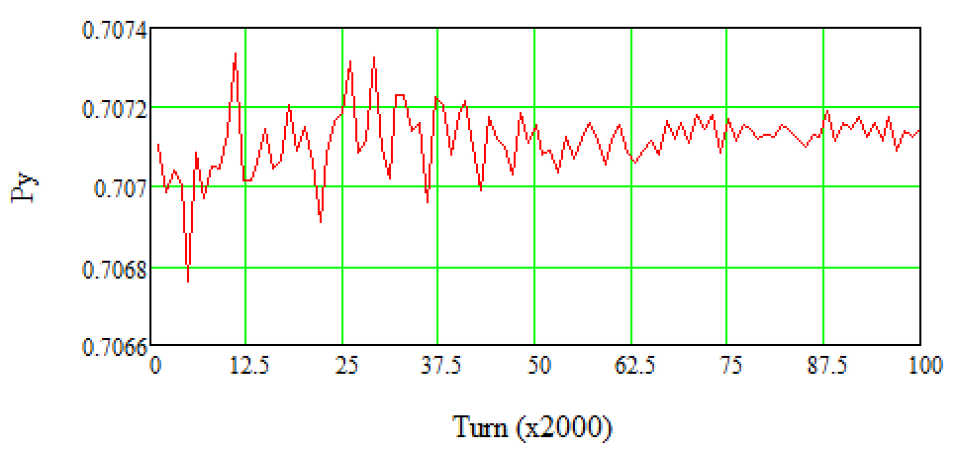
\includegraphics[width=0.9\linewidth]{2_polar2} \\ а)
    \end{minipage}
    \hfill
    \begin{minipage}[b][][b]{0.49\linewidth}\centering
        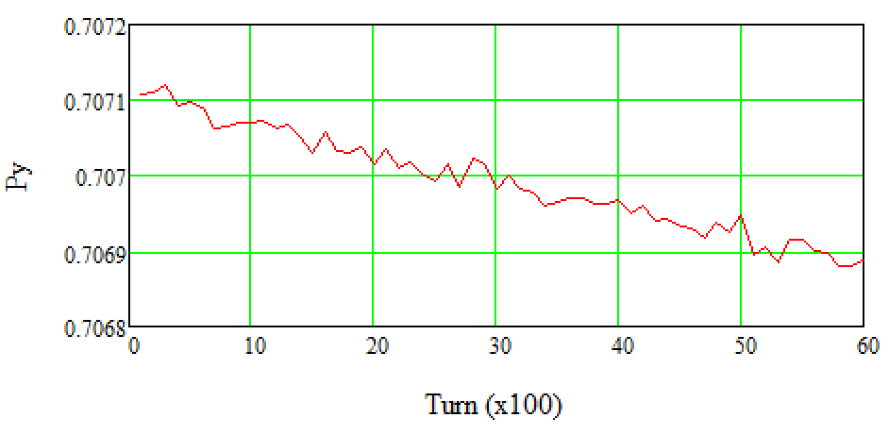
\includegraphics[width=0.9\linewidth]{2_polar1} \\ б)
    \end{minipage}
    \caption{Изменение поляризации во время процедуры скачка критической энергии: (а) ускорение на этапе 2, (б) скачок на этапе 3.}
    \label{fig:polar}
\end{figure}

\par При моделировании рассматриваются частицы с различными доступными начальными параметрами. На рис. \ref{fig:polar} показано изменение поляризации на 2-м ($2\times10^5$ оборотов) и 3-м ($6\times10^3$ оборота) этапах процедуры скачка критической энергии. Поляризация здесь определяется как сумма проекций вектора спина на ось Y всех частиц и существенно не менялась в ходе процедуры. Стоит отметить, что COSY Infinity позволяет отслеживать вектор спина только для небольшого числа частиц, а не для ансамбля, что является существенным для изучения поляризации.

\par Более подробно спиновая динамика будет рассмотрена в ЭДМ-эксперименте всего комплекса NICA-Nuclotron в Главе \ref{ch:EDM}.

\section*{Выводы}
\par Рассмотрена продольная динамика пучка вблизи критической энергии, а также при её пересечении. Такая особенность характерна для структуры, в которой энергия инжекции пучка меньше критической энергии установки и возникает необходимость её преодоления для ускорения до конечной энергии эксперимента.

\begin{enumerate}

\item Воздействие критической энергии на продольную динамику пучка вызывает увеличение фазового объёма в результате неадиабатичности и нелинейности движения в области энергии, близкой к критической;

\item Для преодоления критической энергии может быть применена процедура скачка, которая подразумевает кратковременное изменение дисперсионной функции. Это может быть достигнуто путём использования дополнительных квадруполей или квадруполей поворотной арки. В первом случае можно добиться сохранения частоты, а во втором — необходимо контролировать изменение рабочей точки и стабильность в поперечной плоскости. Таким образом, определяется величина и темп изменения критической энергии при проведении процедуры скачка;

\item Тип ВЧ (Гармонический или барьерный) оказывает влияние на темп ускорения, а также на продольное распределение внутри сепаратрисы. В сочетании со схемой процедуры скачка, необходимо сравнивать темп изменения критической энергии таким образом, чтобы относительный темп при пересечении критической энергии был в разы выше темпа ускорения;

\item Проведено исследование влияния простейших моделей импедансов на динамику. Результаты показали, что для интенсивных сгустков влияние импедансов оказывается значительным. Применение более точных моделей импедансов может существенно углубить понимание реальной динамики системы;

\item В условиях, близких к критическим для интенсивного пучка, развивается продольная микроволновая неустойчивость, которая существенно ограничивает характеристики пучка в конечном эксперименте и, в результате приводит к уменьшению светимости в коллайдере.

\end{enumerate}


\FloatBarrier
